\documentclass[12pt,a4paper]{article}
\usepackage[utf8]{inputenc}
\usepackage[portuguese]{babel}
\usepackage{graphicx}
\usepackage{subcaption}
\usepackage{geometry}
\usepackage{booktabs}
\usepackage{tabularx}
\usepackage{hyperref}
\usepackage{float}
\usepackage{longtable}
\usepackage{array}
\usepackage{indentfirst}
\usepackage[table]{xcolor}
\usepackage{makecell}
\usepackage{fontawesome5}
\usepackage{todonotes}
\usepackage{listings}
\usepackage{tikz}
\usepackage{enumitem}
\usetikzlibrary{positioning, arrows.meta, shapes.geometric, fit, backgrounds, calc}

\geometry{a4paper, margin=2cm}

\hypersetup{
    colorlinks=true,
    linkcolor=black,
    urlcolor=blue,
    citecolor=black
}

\title{\textbf{Atividade 4 - Projeto e Arquitetura de Software}\\
\large MC656 - Engenharia de Software}
\author{
  Caio Lima Albuquerque - RA: 288808 \\
  Giovana Jacome Marchetti - RA: 177700 \\
  Julia de Souza Nardo - RA: 281272 \\
  Leonardo Carvalho De Luca - RA: 288820\\
  Samuel Rodrigues Ferreira - RA: 195440
}
\date{\today}

\begin{document}

\maketitle

\section{Introdução}
Este documento apresenta a documentação arquitetural e a evolução do design do sistema de votação em três contextos (Eleição Preferencial Australiana, Assembleia do CACo e \textit{Blood on the Clocktower} (BotC)), consolidando a entrega da Atividade 4. O trabalho contempla o mapeamento da arquitetura em nível de componentes (C4 Nível 3), as decisões arquiteturais tomadas na transição para a interface Web com FastAPI, a aplicação de dois padrões de projeto GoF para solucionar problemas reais de acoplamento e criação de objetos, e a análise e refatoração de \textit{code smells} com auxílio de análise estática (SonarCloud e Ruff), preservando integralmente o comportamento verificado pela suíte de testes automatizados. \newline


\textbf{Rastreabilidade e Versão Avaliada no GitHub:}
\begin{itemize}
    \item \textbf{Repositório:} \href{https://github.com/GiizAzul/MC656}\faGithub\texttt{ https://github.com/GiizAzul/MC656}
    \item \textbf{Tag da Versão Avaliada:} \texttt{a4-v1.0.0}
    \item \textbf{Filtro de Issues e PRs:} Todas as issues e Pull Requests desta entrega estão identificados com a label \texttt{Atividade4}.
\end{itemize}

\section{Arquitetura do Sistema}

\subsection{Diagrama C4 --- Nível de Componentes (Nível 3)}
A Figura \ref{fig:c4_componentes} apresenta o diagrama C4 em nível de componentes (Nível 3) do contêiner da Aplicação Web/API construída sobre o framework \textit{FastAPI}, detalhando como os controladores HTTP, dependências transversais, serviços de segurança e motores de domínio interagem entre si.

\begin{figure}[H]
\centering
\begin{tikzpicture}[
    scale=0.8, transform shape,
    node distance=1.2cm and 0.8cm,
    font=\sffamily\footnotesize,
    person/.style={rectangle, rounded corners=5pt, draw=blue!80!black, fill=blue!10, thick, minimum width=4.2cm, minimum height=1.2cm, align=center, inner sep=4pt},
    component/.style={rectangle, rounded corners=3pt, draw=cyan!70!black, fill=cyan!10, thick, minimum width=3.3cm, minimum height=1.5cm, align=center},
    dom/.style={
        rectangle, rounded corners=3pt, draw=teal!80!black, fill=teal!10, thick,
        text width=3.4cm, minimum height=2.0cm, align=center, inner sep=4pt
    },
    boundary/.style={
        rectangle, dashed, draw=gray!70!black, very thick, inner sep=10pt, rounded corners=6pt, minimum width=16cm
    },
    lbl/.style={font=\sffamily\tiny, fill=white, inner sep=1.5pt, text=black!85},
    router/.style={
        rectangle, rounded corners=3pt, draw=cyan!75!black, fill=cyan!10, thick,
        text width=3.4cm, minimum height=1.9cm, align=center, inner sep=4pt
    },
    shared/.style={
        rectangle, rounded corners=3pt, draw=orange!80!black, fill=orange!10, thick,
        text width=6.8cm, minimum height=1.3cm, align=center, inner sep=4pt
    },
    arrow/.style={-{Stealth[length=2.2mm]}, thick, draw=gray!80!black},
    bus/.style={-{Stealth[length=2.2mm]}, semithick, dashed, draw=orange!85!black},
]

% 1. Ator (Topo centralizado)
\node[person] (user) at (0, 0) {
    \textbf{\footnotesize Usuário do Sistema} \quad (Person)\\[2pt]
    Navegador Web (Eleitor, Candidato, Estudante, Gestão, Jogador ou Storyteller)
};
% 2. Camada de Entrada e Roteadores FastAPI
\node[component, below=1.6cm of user, xshift=-5.8cm] (auth_router) {\textbf{Auth Router}\\ \scriptsize [FastAPI \texttt{APIRouter}]\\ \scriptsize \texttt{/login}, \texttt{/cadastro},\\ \scriptsize \texttt{/dashboard}, \texttt{/admin}};

\node[component, right=0.6cm of auth_router] (aus_router) {\textbf{Australia Router}\\ \scriptsize [FastAPI \texttt{APIRouter}]\\ \scriptsize \texttt{GET/POST /australia/votar}};

\node[component, right=0.6cm of aus_router] (caco_router) {\textbf{CACo Router}\\ \scriptsize [FastAPI \texttt{APIRouter}]\\ \scriptsize \texttt{/assembleia}, \texttt{/votar},\\ \scriptsize \texttt{/iniciar}, \texttt{/encerrar}, \texttt{/resultados}};

\node[component, right=0.6cm of caco_router] (botc_router) {\textbf{BotC Router}\\ \scriptsize [FastAPI \texttt{APIRouter}]\\ \scriptsize \texttt{/partida}, \texttt{/votar},\\ \scriptsize \texttt{/registrar}, \texttt{/apurar}};

% 3. Camada Transversal (Middleware / Guard & View Engine)
\node[component, below=1.5cm of auth_router, xshift=1.8cm, minimum width=5.0cm] (deps) {\textbf{Auth Guard / Dependências}\\ \scriptsize [FastAPI \texttt{Depends}]\\ \scriptsize \texttt{obter\_usuario\_logado} (Valida Cookie \texttt{HttpOnly/Secure})};

\node[component, below=1.5cm of caco_router, xshift=1.8cm, minimum width=5.0cm] (views) {\textbf{View Engine (SSR)}\\ \scriptsize [\texttt{Jinja2Templates} + CSS]\\ \scriptsize Renderiza \texttt{*.html} e \texttt{style.css}};

% 4. Camada de Serviços e Domínio (Fundo)
\node[dom, below=1.6cm of deps, xshift=-1.8cm] (auth_srv) {\textbf{Serviço de Autenticação}\\ \scriptsize [\texttt{src/autenticacao/}]\\ \scriptsize \texttt{ServicoAutenticacao}, \texttt{UUID v4},\\ \scriptsize Mapa Username/RA e Escopos};

\node[dom, right=0.6cm of auth_srv] (aus_dom) {\textbf{Motor Austrália}\\ \scriptsize [\texttt{src/australia.py}]\\ \scriptsize \texttt{EleicaoAustralia}\\ \scriptsize (Voto Preferencial / IRV)};

\node[dom, right=0.6cm of aus_dom] (caco_dom) {\textbf{Motor CACo}\\ \scriptsize [\texttt{src/caco.py}]\\ \scriptsize \texttt{EleicaoAssembleia}\\ \scriptsize (Estados, Quórum e Urna)};

\node[dom, right=0.6cm of caco_dom] (botc_dom) {\textbf{Motor BotC}\\ \scriptsize [\texttt{src/botc.py}]\\ \scriptsize \texttt{SistemaEleitoralBotC}\\ \scriptsize (Forca, Maioria e Empates)};

% Contorno do Container (Boundary C4) e Título separado (evita bug do pgfkeys com ':')
\begin{scope}[on background layer]
    \node[boundary, fit=(auth_router) (botc_router) (deps) (views) (auth_srv) (botc_dom)] (container) {};
\end{scope}
\node[anchor=north west, font=\sffamily\bfseries\footnotesize, text=gray!80!black] at (container.south west) {Container --- Aplicação Web \& Core (\texttt{src/main.py} --- FastAPI / Python 3.12)};

% Relacionamentos (Setas)
% Usuário -> Routers
\draw[arrow] (user.south) -- ++(0,-0.55) -| node[lbl, pos=0.25] {HTTPS GET/POST} (auth_router.north);
\draw[arrow] (user.south) -- ++(0,-0.55) -| (aus_router.north);
\draw[arrow] (user.south) -- ++(0,-0.55) -| (caco_router.north);
\draw[arrow] (user.south) -- ++(0,-0.55) -| (botc_router.north);

% Routers -> Dependências e Views
\draw[arrow] (auth_router.south) -- (deps.north -| auth_router.south);
\draw[arrow] (aus_router.south) -- (deps.north -| aus_router.south);
\draw[arrow] (caco_router.south) -- (deps.north);
\draw[arrow] (botc_router.south) -- (deps.north);

\draw[arrow] (auth_router.south) -- (views.north);
\draw[arrow] (aus_router.south) -- (views.north);
\draw[arrow] (caco_router.south) -- (views.north -| caco_router.south);
\draw[arrow] (botc_router.south) -- (views.north);

% Dependências e Routers -> Domínio
\draw[arrow] (deps.south) -- node[lbl] {Valida Sessão} (auth_srv.north);
\draw[arrow] (auth_router.south west) to[out=-105, in=115] node[lbl, pos=0.8] {Login / Cadastro} (auth_srv.north west);

\draw[arrow] (aus_router.south) to[out=-10, in=75] (aus_dom.north east);

\draw[arrow] (caco_router.south) to[out=-150, in=115] (caco_dom.north);

\draw[arrow] (botc_router.south) to[out=-10, in=70] (botc_dom.north east);

\end{tikzpicture}
\caption{Diagrama C4 em Nível de Componentes (Nível 3) da Aplicação Web.}
\label{fig:c4_componentes}
\end{figure}

\subsection{Principais Componentes, Responsabilidades e Relações}
A arquitetura interna do sistema é modularizada para separar os protocolos de interface das regras matemáticas de apuração e controle de elegibilidade. A Tabela \ref{tab:componentes} descreve cada componente presente na implementação atual (`src/').

\renewcommand{\arraystretch}{1.4}
\begin{longtable}[H]{|m{3.5cm}|m{6.5cm}|m{5cm}|}
\hline
\centering
\small
\textbf{Componente} & \textbf{Arquivos (\texttt{src/})} & \textbf{Responsabilidades e Relações} \\
\hline
\textbf{Bootstrap \& State} & \texttt{main.py} & Ponto de entrada da aplicação FastAPI. Inicializa as instâncias singleton em memória (\texttt{app.state}), monta os arquivos estáticos (\texttt{/static}), registra os roteadores e intercepta exceções globais de sessão. \\
\hline
\textbf{Auth Router} & \texttt{routers/auth\_router.py} & Gerencia autenticação (\texttt{/login}, \texttt{/logout}), criação de contas (\texttt{/cadastro}) e renderização dos painéis (\texttt{/dashboard}, \texttt{/admin}). Consome o \textit{Serviço de Autenticação} e atualiza a lista de eleitores ativos. \\
\hline
\textbf{Australia Router} & \texttt{routers/australia\_router.py} & Controla a exibição da cédula preferencial (\texttt{GET /australia/votar}) e processa o envio do ranking (\texttt{POST /australia/votar}), validando sequencialidade (1 a $N$) e unicidade de voto por eleitor antes de repassar ao motor de domínio. \\
\hline
\textbf{CACo Router} & \texttt{routers/caco\_router.py} & Gerencia o fluxo da assembleia estudantil (\texttt{/caco/assembleia}, \texttt{/votar}, \texttt{/iniciar}, \texttt{/encerrar}, \texttt{/resultados}). Restringe comandos de condução ao escopo \texttt{CACO\_GESTAO} e interage com o motor \texttt{EleicaoAssembleia}. \\
\hline
\textbf{BotC Router} & \texttt{routers/botc\_router.py} & Expõe as rotas da partida (\texttt{/botc/partida}, \texttt{/votar}) e ações exclusivas do Mestre (\texttt{/registrar}, \texttt{/apurar}), delegando a lógica ao \texttt{SistemaEleitoralBotC}. \\
\hline
\textbf{Middleware / Auth Guard} & \texttt{routers/dependencias.py} & Componente transversal injetado via \texttt{Depends} (\texttt{obter\_usuario\_logado}). Extrai o cookie \texttt{sessao\_usuario}, resolve o objeto \texttt{Usuario} no banco em memória e dispara \texttt{RequerRedirecionamento Exception} em acessos não autenticados. \\
\hline
\textbf{View Engine (SSR)} & \texttt{templates/*.html} \newline \texttt{static/style.css} & Camada de apresentação baseada em templates \textit{Jinja2} com herança de layout (\texttt{base.html}) e estilização centralizada via CSS semântico. \\
\hline
\textbf{Serviço de Autenticação e Autorização} & \texttt{autenticacao/base.py} \newline \texttt{autenticacao/autorizacao.py} \newline \newline \texttt{autenticacao/caco.py autenticacao/botc.py autenticacao/australia.py} & Mantém o repositório de contas indexado por \texttt{UUID v4} (\texttt{\_banco\_por\_id}) e mapeamento duplo por \texttt{username} e \texttt{RA} (\texttt{\_mapa\_usernames}). Define a hierarquia polimórfica de usuários e valida permissões por escopo (\texttt{MACRO\_SCOPES}). \\
\hline
\textbf{Motores de Domínio Eleitoral} & \texttt{australia.py} \newline \texttt{caco.py} \newline \texttt{botc.py} \newline \texttt{interfaces.py} & Núcleo de regras de negócio puras, independentes de I/O: \texttt{EleicaoAustralia} (transferência iterativa de votos e eliminação), \texttt{EleicaoAssembleia} (máquina de estados, quórum de 10\% e contagem anônima) e \texttt{SistemaEleitoralBotC} (regras de maioria na forca e empate). \\
\hline
\caption{Principais componentes da arquitetura e suas responsabilidades.}
\label{tab:componentes}
\end{longtable}

\subsection{Estilos Arquiteturais Adotados}
A estrutura da aplicação combina dois estilos arquiteturais complementares:

\begin{enumerate}
    \item \textbf{Arquitetura em Camadas (\textit{Layered Architecture}) com padrão MVC Server-Side Rendered (SSR):} A aplicação separa claramente a \textbf{Camada de Apresentação} (Templates Jinja2 + CSS), a \textbf{Camada de Controle e Roteamento HTTP} (Roteadores FastAPI e Guardas de Dependência) e a \textbf{Camada de Domínio e Serviços} (`src/australia.py`, `src/caco.py`, `src/botc.py`, `src/autenticacao/`). As dependências fluem estritamente de cima para baixo: os motores de domínio não conhecem objetos HTTP (`Request`, `Form`, `Cookie`) nem comandos de terminal (`input`/`print`), o que permitiu manter a compatibilidade simultânea entre a antiga interface CLI e a nova interface Web.
    \item \textbf{Arquitetura Modular Orientada a Domínios (\textit{Vertical Slices} nos Controladores):} Na camada de roteamento e de visualização, os componentes são particionados verticalmente pelos três contextos de negócio (\texttt{australia\_router}, \texttt{caco\_router}, \texttt{botc\_router}) apoiados por um módulo transversal de autenticação e autorização (\texttt{auth\_router} e \texttt{dependencias}).
\end{enumerate}

\subsection{Decisões Arquiteturais Relevantes (ADRs)}

\subsubsection*{Decisão 1: Desacoplamento do Domínio e Coexistência de Múltiplas Interfaces (Web SSR com FastAPI/Jinja2 + CLI)}
\begin{itemize}
    \item \textbf{Contexto e Justificativa:} Na Atividade 2, o sistema operava exclusivamente via terminal (CLI). Com a elicitação de requisitos da Atividade 3, surgiu a necessidade de usabilidade para usuários leigos via navegador (Web). Em vez de reescrever as regras de negócio ou criar uma SPA complexa em JavaScript separado (React/Vue), a equipe decidiu manter os motores de domínio puros em Python e introduzir o \textit{FastAPI} acoplado ao motor de templates \textit{Jinja2} (Server-Side Rendering).
    \item \textbf{Consequências e Trade-offs:}
    \begin{itemize}
        \item \textit{Positivas:} Reaproveitamento integral (100\%) dos testes de unidade de domínio já existentes; simplicidade de deploy em um único processo Python; ausência de problemas de CORS; e facilidade de testar o fluxo completo de ponta a ponta usando o \texttt{TestClient} do Starlette/FastAPI (atingindo 100\% de cobertura nos roteadores).
        \item \textit{Negativas / Trade-offs:} A renderização no servidor exige recarregamento de página a cada submissão de formulário (\texttt{POST} $\rightarrow$ \texttt{TemplateResponse}/\texttt{RedirectResponse}), oferecendo menor interatividade em tempo real do que uma arquitetura baseada em WebSockets ou SPA para atualizações automáticas de placar.
    \end{itemize}
\end{itemize}

\subsubsection*{Decisão 2: Gestão de Estado Centralizada em Memória (\texttt{app.state}) e Sessão via Cookies \texttt{HttpOnly} com Injeção de Dependências}
\begin{itemize}
    \item \textbf{Contexto e Justificativa:} O sistema precisava garantir persistência de sessão entre múltiplas votações, impedir votos duplicados e isolar os escopos de permissão (Eleitor, Candidato, Estudante, Gestão, Jogador e Storyteller) sem introduzir a sobrecarga de configuração de um SGBD relacional externo nesta etapa do projeto. Decidiu-se centralizar o estado no objeto \texttt{app.state} do FastAPI, indexar usuários internamente por \texttt{UUID v4} imutável (com índice secundário por \texttt{username} e \texttt{RA}) e gerenciar a sessão por meio de cookies \texttt{HttpOnly} validados por injeção de dependência (\texttt{Annotated[Usuario, Depends(obter\_usuario\_logado)]}).
    \item \textbf{Consequências e Trade-offs:}
    \begin{itemize}
        \item \textit{Positivas:} Proteção contra acesso a cookies via scripts maliciosos no navegador (\texttt{httponly=True}); padronização da verificação de autenticação fora do corpo das rotas (evitando código morto e duplicação); altíssima velocidade de execução dos 180 testes automatizados sem necessidade de \textit{containers} de banco de dados.
        \item \textit{Negativas / Trade-offs:} Como o estado reside na memória RAM do processo Uvicorn (\texttt{app.state}), o reinício do servidor apaga os votos e cadastros dinâmicos, e a aplicação não pode ser escalada horizontalmente com múltiplos \textit{workers} sem antes migrar o estado para um armazenamento compartilhado (como Redis ou PostgreSQL).
    \end{itemize}
\end{itemize}


\section{Padrões de Projeto}

Para evoluir o design interno da aplicação e reduzir o acoplamento identificado durante a expansão para a Web, foram selecionados e implementados dois padrões de projeto clássicos (GoF) voltados a problemas reais do código.

\subsection{Aplicação 1: Padrão Criacional --- \textit{Factory Method / Simple Factory} na Criação Polimórfica de Usuários}

\begin{table}[H]
\centering
\small
\begin{tabularx}{\textwidth}{|l|X|}
\hline
\textbf{Problema Identificado} & 
Violação do Princípio Aberto-Fechado (OCP). O controlador Web (\texttt{src/routers/auth\_router.py}, na função \texttt{processar\_cadastro}) possuía cadeias extensas de \texttt{if/elif/else} verificando strings (\texttt{"CACO\_ESTUDANTE"}, \texttt{"CACO\_GESTAO"}, \texttt{"AUSTRALIA\_ELEITOR"}, etc.), validando regras específicas (como a obrigatoriedade numérica do RA para estudantes) e instanciando diretamente as 6 subclasses concretas de \texttt{Usuario}. \\
\hline
\textbf{Padrão Escolhido e Justificativa} & 
\textbf{Simple Factory / Factory Method} (\texttt{UsuarioFactory}). A criação polimórfica de contas foi encapsulada em uma fábrica dedicada na camada de autenticação (\texttt{src/autenticacao/}). O padrão é ideal porque centraliza as regras de validação de parâmetros de criação (como conversão e checagem do RA) e desacopla os controladores Web das classes concretas de cada domínio eleitoral. \\
\hline
\textbf{Consequências da Solução} & 
\begin{itemize}[leftmargin=1em, nosep]
    \item \textbf{Positivas:} Redução drástica da Complexidade Cognitiva na rota \texttt{POST /cadastro}; facilidade para adicionar novos perfis de usuário em um único ponto do sistema.
    \item \textbf{Negativas:} Introdução de mais uma classe/estrutura na camada de autenticação.
\end{itemize} \\
\hline
\textbf{Rastreabilidade no GitHub} & 
\begin{itemize}[leftmargin=1em, nosep]
    \item \textbf{Issue:} \href{https://github.com/GiizAzul/MC656/issues/94}{Refatoração da instanciação de usuários com o padrão Simple Factory \#94}
    \item \textbf{Pull Request:} \href{https://github.com/GiizAzul/MC656/pull/95}{Refactor: Implementar padrão Simple Factory no cadastro de usuários
\#95}
\end{itemize} \\
\hline
\end{tabularx}
\caption{Especificação da primeira aplicação de padrão de projeto.}
\end{table}

\begin{table}[H]
\centering
\small
\begin{tabularx}{\textwidth}{|l|X|}
\hline
\textbf{Problema Identificado} &
No módulo \texttt{src/caco.py} (\texttt{EleicaoAssembleia}), o controle do ciclo de votação utilizava o atributo \texttt{estado}, representado anteriormente por valores de um \texttt{Enum}, além de verificações condicionais para controlar as operações de início, registro de votos e encerramento. Parte das regras de controle também era distribuída entre a classe de domínio e o roteador, dificultando a centralização das transições de estado e a manutenção do código. \\
\hline

\textbf{Padrão Escolhido e Justificativa} &
\textbf{Padrão State}. Foram criadas classes para representar os estados de espera, votação em andamento e votação encerrada, definidas em \texttt{src/estados.py}. A abstração \texttt{SistemaEleitoral}, em \texttt{src/interfaces.py}, passou a delegar as operações de início, registro de votos e encerramento ao estado atual. A implementação de \texttt{EleicaoAssembleia} foi adaptada para utilizar essa estrutura, e o roteador do CACo foi atualizado para trabalhar com a nova representação dos estados. Dessa forma, os comportamentos e as transições da votação passam a ser organizados de acordo com o estado ativo. \\
\hline

\textbf{Consequências da Solução} &
\begin{itemize}[leftmargin=1em, nosep]
    \item \textbf{Positivas:} Encapsulamento dos comportamentos associados a cada estado; centralização das transições da votação; redução do acoplamento entre a lógica de domínio e o roteador; maior facilidade de manutenção e extensão para os demais contextos; possibilidade de rejeitar operações incompatíveis com o estado atual por meio de exceções \texttt{RuntimeError}.
    \item \textit{Negativas:} Aumento do número de classes para representar os estados e necessidade de adaptar a interface \texttt{SistemaEleitoral} e os componentes dependentes da representação anterior.
\end{itemize} \\
\hline

\textbf{Rastreabilidade no GitHub} &
\begin{itemize}[leftmargin=1em, nosep]
    \item \textbf{Issue:} \href{https://github.com/GiizAzul/MC656/issues/91}{Refatorar o controle de estados da votação utilizando o padrão State \#91}
    \item \textbf{Pull Request:} \href{https://github.com/GiizAzul/MC656/pull/92}{Refatora o controle de estados da votação do CACo com o padrão State \#92}
\end{itemize} \\
\hline
\end{tabularx}
\caption{Especificação da segunda aplicação de padrão de projeto.}
\end{table}


\section{Code Smells e Refatoração}

Com o auxílio da ferramenta de análise estática contínua \textbf{SonarCloud} integrada ao repositório e do linter \textbf{Ruff}, o código foi inspecionado em busca de \textit{code smells} e \textit{design smells}. A seguir, documentamos duas ocorrências de tipos distintos identificadas no sistema.

\begin{figure}[H]
    \centering
    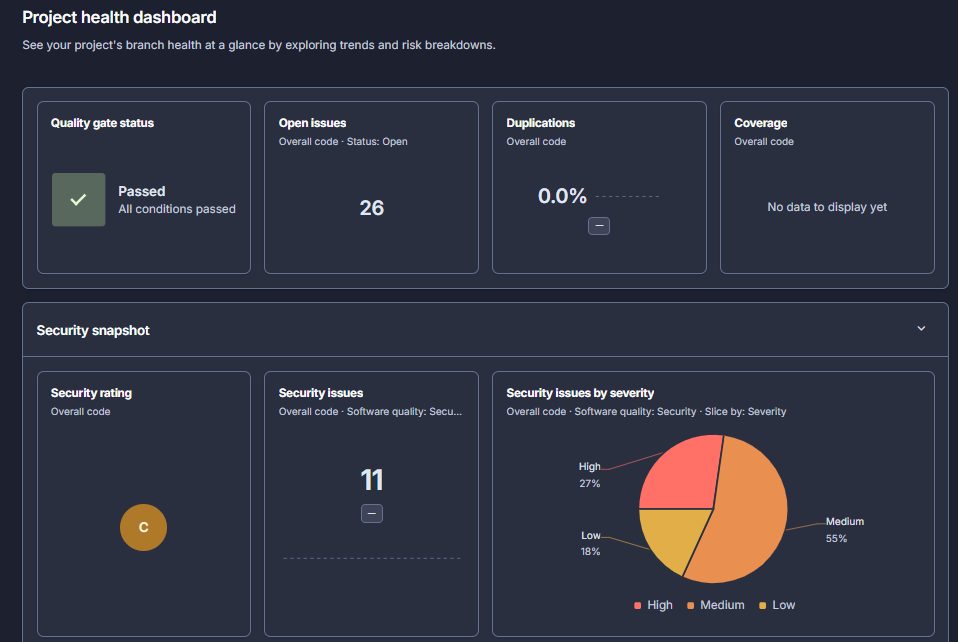
\includegraphics[width=0.8\linewidth]{imagens/sonarcloud_dashboard.png}
    \caption{Ilustração do dashboard do SonarCloud}
    \label{fig:sonar_cloud_dashboard}
\end{figure}

\subsection{Ocorrência 1: Controles de Formulário Desacoplados de Rótulos Semânticos (\texttt{Web:S6853} e \texttt{Web:InputWithoutLabelCheck})}
\begin{itemize}
    \item \textbf{Localização:} \texttt{src/templates/cadastro.html}, \texttt{src/templates/admin.html} e \\ \texttt{src/templates/australia.html}.
    \item \textbf{Smell Identificado:} \textbf{Ausência de associação explícita entre rótulos (\texttt{<label>}) e controles de entrada (\texttt{<input>}, \texttt{<select>})} --- Regras SonarCloud \texttt{Web:S6853} (\textit{Label elements should have a text label and an associated control}) e \texttt{Web:InputWithoutLabelCheck} (\textit{Input, select and textarea tags should be labeled}).
    \item \textbf{Justificativa:} Nos templates Jinja2 da camada de visualização, as tags \texttt{<label>} foram declaradas apenas visualmente acima dos campos de entrada sem o atributo \texttt{for}, e os elementos \texttt{<input>} e \texttt{<select>} não possuíam identificadores únicos (\texttt{id}). Na tela de votação da Austrália (\texttt{australia.html}), os nomes dos candidatos estavam encapsulados em tags genéricas \texttt{<span>} ao lado dos inputs numéricos de ranqueamento.
    \item \textbf{Impacto na Manutenção e Evolução:} Compromete diretamente os requisitos não funcionais de \textbf{Usabilidade e Acessibilidade} do sistema (tecnologias assistivas e leitores de tela não conseguem identificar qual dado deve ser inserido em cada campo), reduz a área clicável de foco dos formulários em dispositivos móveis e dificulta a seleção determinística de elementos DOM em futuros testes automatizados de interface (\textit{End-to-End}).
\end{itemize}

\subsection{Ocorrência 2: Cookie de Sessão sem Diretiva de Transporte Seguro (\texttt{python:S2092})}
\begin{itemize}
    \item \textbf{Localização:} \texttt{src/routers/auth\_router.py} (função \texttt{processar\_login}).

    \item \textbf{Smell / Hotspot Identificado:} \textbf{Criação de Cookie de Autenticação sem a flag \texttt{secure}} (Regra SonarCloud \texttt{python:S2092}).
    
    \item \textbf{Justificativa:} Nas rotas de login e cadastro, o cookie \texttt{sessao\_usuario} era emitido apenas com \texttt{httponly=True}, omitindo os atributos \texttt{secure=True} e \texttt{samesite="lax"}, mas se um cookie de sessão for enviado por uma conexão HTTP não criptografada, um invasor que conseguir interceptar o tráfego pode roubá-lo. Com um cookie de sessão válido, o invasor pode se passar pela vítima e ter acesso completo à conta dela sem precisar saber a senha. Mesmo em sites que usam principalmente HTTPS, uma única requisição HTTP contendo o cookie de sessão já é suficiente para expô-lo.
    
    \item \textbf{Impacto na Manutenção e Evolução:} A ausência da flag \texttt{secure} expõe o token de sessão a interceptações em conexões não criptografadas (\textit{Man-in-the-Middle}).
\end{itemize}
\subsection{Refatoração Realizada}

\begin{itemize}
    \item \textbf{Ocorrências Refatoradas:} Ambas as ocorrências apontadas pelo SonarCloud e pelo Ruff foram integralmente tratadas para zerar os alertas de qualidade do projeto:
    \begin{enumerate}
        \item \textbf{Refatoração Semântica dos Templates HTML:} Nos arquivos \texttt{cadastro.html} e \texttt{admin.html}, todos os elementos \texttt{<input>} e \texttt{<select>} receberam atributos \texttt{id} semânticos vinculados aos respectivos \texttt{<label for="...">}. Em \texttt{australia.html}, as tags \texttt{<span>} foram convertidas em \texttt{<label for="posicao\_\{\{ loop.index \}\}">} pareadas dinamicamente com cada campo numérico da cédula.
        
        \item \textbf{Endurecimento de Sessão e Tipagem de Dependências:} Nos arquivos\\ \texttt{auth\_router.py}, a emissão do cookie de sessão foi refatorada para incluir \texttt{secure=True} e \texttt{samesite="lax"}.
    \end{enumerate}
    \item \textbf{Preservação do Comportamento:} A suíte completa de \textbf{180 testes automatizados} (\texttt{pytest}) foi executada após as alterações (ajustando o cliente de testes web para operar sobre \texttt{https://testserver}), mantendo 100\% de aprovação e 100\% de cobertura nos roteadores, com zero erros reportados pelo Ruff e pelo SonarCloud.
    \item \textbf{Rastreabilidade no GitHub:}
    \begin{itemize}
        \item \textbf{Issue da Refatoração:}
            \href{https://github.com/GiizAzul/MC656/issues/86}{Correção de code smells de acessibilidade e segurança detectados pelo SonarCloud e Ruff \#86}
        \item \textbf{Pull Request da Refatoração:} \href{https://github.com/GiizAzul/MC656/pull/88}{Refactor: Eliminar code smells do SonarCloud e Ruff \#88}
    \end{itemize}
\end{itemize}

\end{document}